\subsection{Learning of Phrases}
We make use of a semi-automated approach to identify key-phrases for the purpose of extracting events from our data feeds. We use different sets of phrases for News and Twitter. We found that key-phrases provide a more accurate extraction than individual keywords.

Initially, a few seed phrases were obtained manually
with the help of subject matter experts. These phrases were parsed
using a dependency parser and the grammatical relationship between the
core subject word---{\em protest}, {\em manifestación}, {\em Huelga},
etc.---and any accompanying word -- {\em plan}, {\em call}, {\em anunciar} --- was extracted. These grammatical relations serve as extraction patterns as in \cite{riloff2003learning}. Then, we build a corpora by finding out sentences that contain both a future date and the protest or its synonyms in any of the three languages. These sentences are then used as candidates for phrase list expansion. The phrase list is populated by finding phrases that follows the extraction pattern.
The phrase learning is shown in Fig.~/ref{fig:phraselearning}

This final set of phrases, is then cleansed by an expert to get the final set of phrases. Around 122 phrases were obtained for News/Blogs and 

To extend the initial set of phrases, a set of sentences/tweets containing a subject word and a
future time/date expression was collected and parsed.  This set of
sentences was used to expand the set of planned protest phrases by
extracting all keyword combinations that have the same grammatical
relation with respect to the core subject word. The final set of
planned protest phrases is then obtained after a manual revision of
the phrases obtained in the last step.

By this approach, we learned 112 phrases for News/blogs and 156 for tweets.

The learned phrases are then used to filter the incoming stream of Documents (news/blogs/twitter). The phrases matching is done by first splitting the incoming document into sentences and then looking for the presence of each individual word of a key-phrase (by lemma) separated by a pre-fixed maximum offset-distance (set to 3). This methodology greatly increases processing speed.

\begin{figure}
\caption{An Example of Phrase Learning}
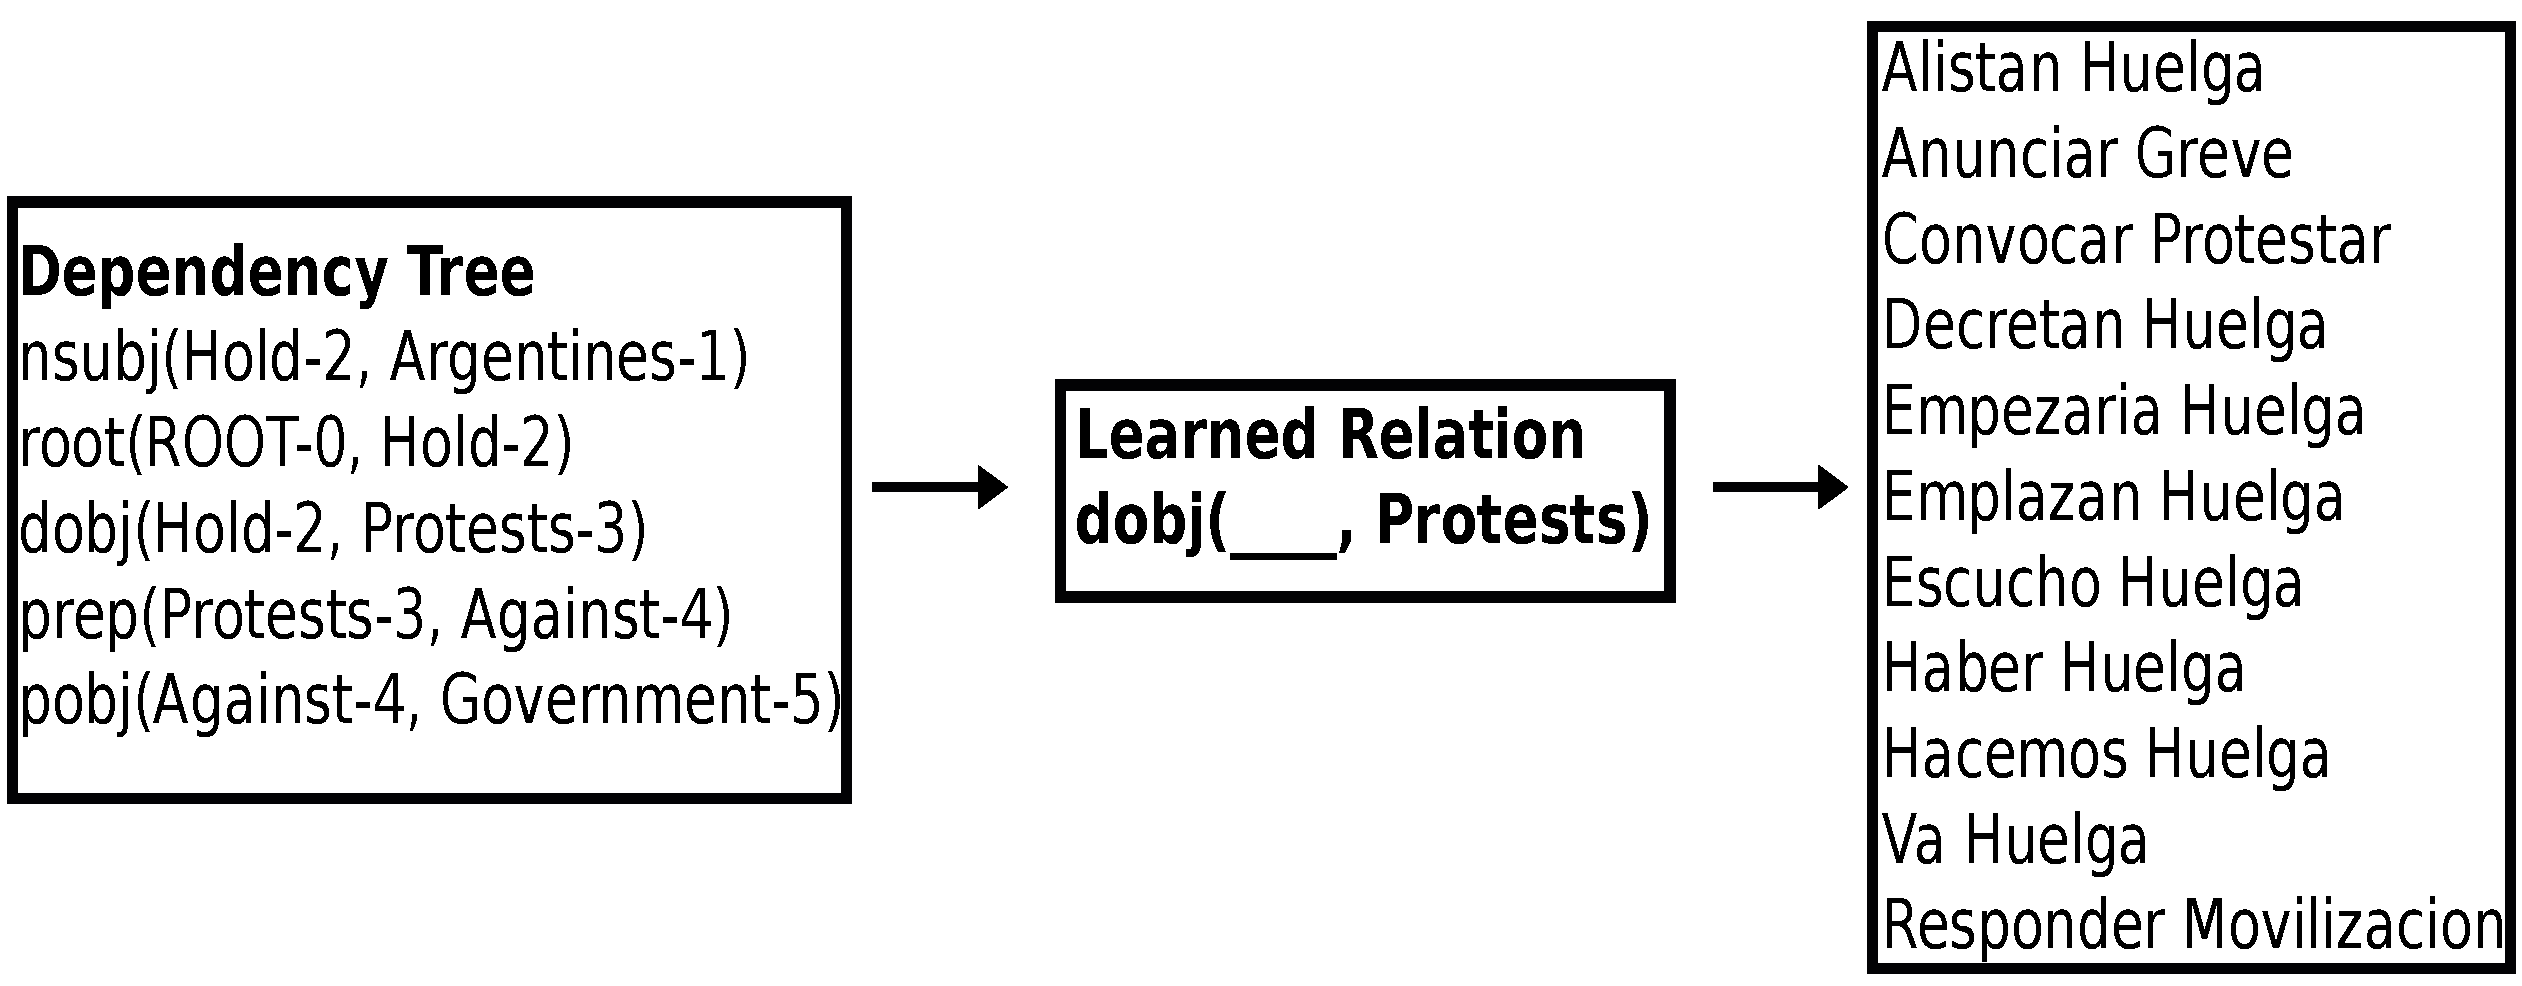
\includegraphics[width=0.5\textwidth]{figures/phraseLearning}
\label{fig:phraseLearning}
\end{figure}



\subsection{classification}
    \sathappanc{Is this Needed? ..We have two classifiers -- Text Based Naive Bayes Classifier for RSS and Facebook. Location Based Classifier for Twitter}

All News,Blogs and Tweets are first searched for the phrases learned. Then the filtered documents are searched for the presence of a reference to a Future Date. In case of News/blogs we search for the Presence of a reference to a Future Date only within the sentence where the phrase was found to reduce error. For tweets, we search the entire tweet for the reference to a future date.

Then, finally, a warning/alert is issued for those documents which contains a location information. In the case of tweets, we found that issuing an alert from just one tweet lead to a lot of wrong alerts. We thus, further filter the tweets by setting a threshold (set to 5) on the number of re-tweets of the tweet under consideration.
